%! Author = joseph
%! Date = 27.04.21
% TODO: save copy as beamer template

\documentclass[a4paper, x11names, svgnames]{beamer}

% -- packages
% encoding, language and fonts, more powerful macros
\usepackage[utf8]{inputenc}
\usepackage[T1]{fontenc}
\usepackage{xargs}
\usepackage{xifthen}
%color
%\usepackage[x11names, svgnames]{xcolor}
% math symbols
\usepackage{amsthm}
\usepackage{amsmath}
\usepackage{amssymb}
\usepackage{amsfonts}
\usepackage{bbding}      % checksymbol
\usepackage{array}       % matrices
\usepackage{multicol}
% roman/ arabic enumeration
% graphics, code
\usepackage{float}
\usepackage{caption}
\usepackage{subcaption}
\usepackage{graphicx}
\usepackage{tikz}
\usepackage{environ}  % to scale tikz to scale
\usepackage{color}
\usepackage{mathtools}
\usepackage{xcolor}

% package options
\usetikzlibrary{patterns}

% -- macros
% Zeichen
\input{~/templates/math_symbols.tex}

% spacing
\newcommand{\offset}{1cm}

% -- enviornments
% english theorem env % TODO: export into single file
\theoremstyle{definition}
\newtheorem*{defn}{Definition}
\theoremstyle{plain}
\newtheorem*{prop}{Proposition}
\theoremstyle{plain}
\newtheorem*{cor}{Corrolary}
%\theoremstyle{remark}
%\newtheorem*{proof}{Proof}

% -- document settings 
\title{Linear Programming}
\subtitle{The Simplex Algorithm}
\author{Joseph Holten}
\date{12.5.2021}

% beamer settings
\usetheme{Hannover}
\usecolortheme{seahorse}
\usefonttheme{professionalfonts}


% beamer pause in align
\makeatletter
\let\save@measuring@true\measuring@true
\def\measuring@true{%
    \save@measuring@true
    \def\beamer@sortzero##1{\beamer@ifnextcharospec{\beamer@sortzeroread{##1}}{}}%
    \def\beamer@sortzeroread##1<##2>{}%
    \def\beamer@finalnospec{}%
}
\makeatother

\begin{document}

% title frame
\frame{\maketitle}

% TOC
\frame{\frametitle{Overview}\tableofcontents}   % TODO: move toc to right
% TODO: better sections

\section[Definitions]{Definition of a Linear Program}\label{sec:def} % TODO: maybe rather called "preliminaries"?

% beamer section titles
\AtBeginSection[]{
    \begin{frame}
        \setcounter{tocdepth}{1}
        \frametitle{Section}
        \tableofcontents[currentsection]
    \end{frame}}

% inutition
\begin{frame}{Linear Program Intuition}
    What is a linear Program? $\Ra$ Optimization of a linear function

    \begin{align*}
        \text{1D:} & \qquad &\text{objective} &= c_1\cdot x_1 \\
        \pause
        \text{2D:} & \qquad  & &= c_1\cdot x_1 + c_2\cdot x_2 \\
    \end{align*}
    \pause
    \center
    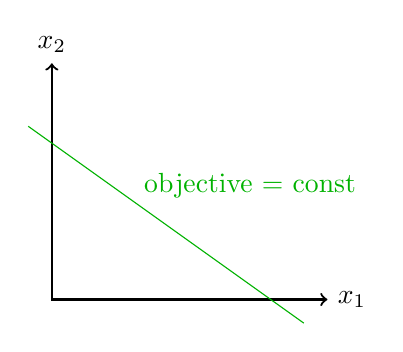
\begin{tikzpicture}
        \draw [<->, thick] (0,3) node (yaxis) [above] {$x_2$} |- (3.5,0) node (xaxis) [right] {$x_1$};
        \draw [black!30!green] (-0.3, 2.2) -- (3.2, -0.3) node [pos=0.35, above, label={right:objective = const}] {};
    \end{tikzpicture}
\end{frame}

% intuition cont.
\begin{frame}{Linear Program Intuition}
        \[c,x \in \R^2\]
        \[\text{objective} = c\cdot x \]
    \pause
    Constraints:
    \begin{overlayarea}{0.45\textwidth}{0.4\textheight}\visible<3->{ % TODO: align constraints vertically
        \[A \in \R^{2\times 2}, b \in \R^2\]
        \[Ax \leq b\]  % TODO: align =
        \[x \geq 0\]
    }\end{overlayarea}%
    \visible<2->{\begin{overlayarea}{0.45\textwidth}{0.5\textheight}  % TODO: single constraints after each other -> system of inequalities = matrix
        \only<2-3>{\center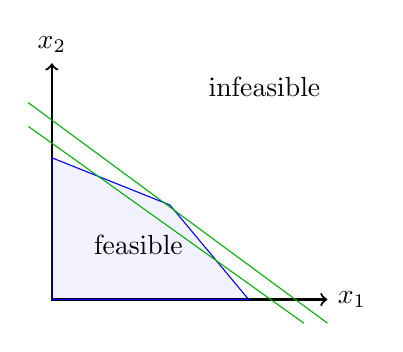
\begin{tikzpicture}
            \draw [<->, thick] (0,3) node (yaxis) [above] {$x_2$} |- (3.5,0) node (xaxis) [right] {$x_1$};
            \draw [blue, fill=blue, fill opacity=0.05] (0.0, 1.8) -- (1.5, 1.2) -- (2.5, 0.0) -- (0,0) -- cycle;
            \draw [black!30!green] (-0.3, 2.2) -- (3.2, -0.3);
            \draw [black!30!green] (-0.3, 2.5) -- (3.5, -0.3); % TODO: make line go through vertex
            \node at (1.1, 0.7) {feasible};   % TODO: opt position of labels
            \node at (2.7, 2.7) {infeasible};
        \end{tikzpicture}}
        % TODO: come in slower
        \only<4>{\center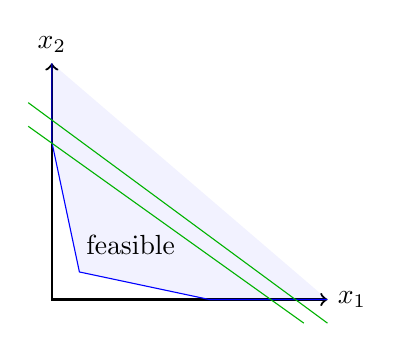
\begin{tikzpicture}  % TODO: slight wobble in picture
             \draw [<->, thick] (0,3) node (yaxis) [above] {$x_2$} |- (3.5,0) node (xaxis) [right] {$x_1$};
             \draw [blue, fill=blue, fill opacity=0.05] (3.5,0) -- (2.0, 0) -- (0.35, 0.35) -- (0, 2.0) -- (0, 3);  % TODO: triangle or rectangle fill?
             \draw [black!30!green] (-0.3, 2.2) -- (3.2, -0.3);
             \draw [black!30!green] (-0.3, 2.5) -- (3.5, -0.3); % TODO: make line go through vertex
             \node at (1, 0.7) {feasible};   % TODO: opt position of labels
        \end{tikzpicture}}
        \only<5>{\center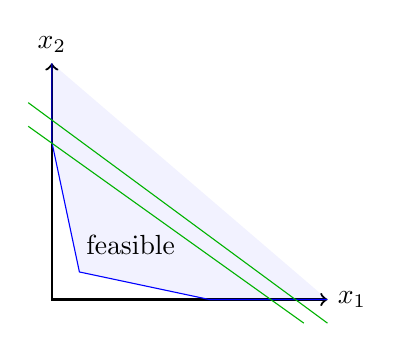
\begin{tikzpicture}  % TODO: slight wobble in picture
             \draw [<->, thick] (0,3) node (yaxis) [above] {$x_2$} |- (3.5,0) node (xaxis) [right] {$x_1$};
             \draw [blue, fill=blue, fill opacity=0.05] (3.5,0) -- (2.0, 0) -- (0.35, 0.35) -- (0, 2.0) -- (0, 3);  % TODO: triangle or rectangle fill?
             \draw [black!30!green] (-0.3, 2.2) -- (3.2, -0.3);
             \draw [black!30!green] (-0.3, 2.5) -- (3.5, -0.3); % TODO: make line go through vertex
             \node at (1, 0.7) {feasible};   % TODO: opt position of labels
        \end{tikzpicture}}
    \end{overlayarea}}
\end{frame}

% 3D example
\begin{frame}{Linear Program Intuition}
    In 3D:
    TODO (tikz picture in 3D?)

\end{frame}

% definition
\begin{frame}{Linear Program Definition}
    \begin{defn}[Linear Program]
        A \textbf{Linear Program (LP)} is the following optimization problem: \\
        \vspace*{0.3cm}
        \hspace*{0.5cm}Given $A \in \R^{n\times m}, b \in \R^m, c\in\R^n$  \\
        %\vspace*{0.7cm}
        \hspace*{1.5cm}  % TODO: position table
        \begin{tabular}{l l}
            find        & $x \in\R^n$  \\  % TODO: possible center aligned text in 2nd column
            maximizing  & $c\cdot x$   \\
            s.t.        & $Ax \leq b$  \\
        \end{tabular} \\
        \pause
        \vspace{0.3cm}
        Special cases: \\
        \begin{itemize}
            \item $\{x\st Ax\leq b\}$ empty
            \item unbounded: $\forall\alpha\in\R\,\exists x\in\R^n\st c\cdot x > \alpha$
        \end{itemize}
        The set $\{x \st Ax \leq b\}$ is called a \textbf{polyhedron}.
        A bounded polyhedron called a polytope.
    \end{defn}
\end{frame}

% feasible + bounded => has opt
\begin{frame}{Existance of Optimum}
    \begin{theorem}
        If a Linear Program is feasible and bounded, there is a vector attaining the maximum. \\
        \pause
        Formally: For $P=\{x\in\R^n\st Ax\leq b\}\neq\emptyset$ and $c\in\R^n$
        with $\delta\coloneqq\sup\{c\cdot x\st x\in P\} < \infty$. Then there exists a vector $z\in P$
        with $\delta = c\cdot z$.
    \end{theorem}
\end{frame}

\subsection{Polyhedra}
% properties of polyhedra
\begin{frame}{Properties of Polyhedra (WIP)}
    % definitions
    \begin{minipage}[l]{0.6\textwidth}
    \begin{defn}
        Let $P\coloneqq\{x\st Ax \leq b\}$ be a (non empty) polyhedron.
        \begin{itemize}
            \item<2-> For $c\in\R^n \setminus \{0\}$ with $\delta \coloneqq\max\{c\cdot x\st x\in P\}$ finite,
                      then $\{x\st c\cdot x = \delta\}$ is a supporting \textbf{hyperplane}.
            \item<3-> $P \cap \text{hyperplane}$ is a \textbf{face}.
            \item<4-> If $\{x\}$ is a face, x is called a \textbf{vertex}.
        \end{itemize}
    \end{defn}
    \end{minipage}
    % picture
    \begin{minipage}[r]{0.35\textwidth}
        \resizebox{\textwidth}{!}{
        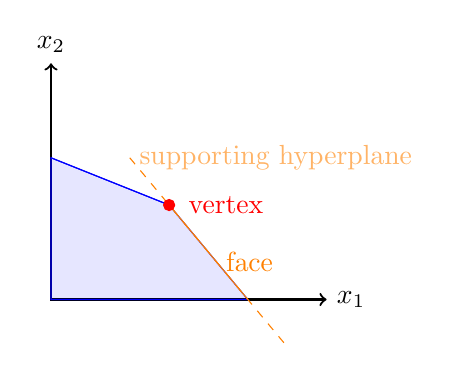
\begin{tikzpicture} % TODO: overlapping lines not pretty
            % axis
            \draw [<->, thick] (0,3) node (yaxis) [above] {$x_2$} |- (3.5,0) node (xaxis) [right] {$x_1$};
            % polygon
            \draw  [blue, fill=blue, fill opacity=0.05] (0.0, 1.8) -- (1.5, 1.2) -- (2.5, 0.0) -- (0,0) -- cycle;
            % polygon missing one side
            \draw<2-> [blue] (0.0, 1.8) -- (1.5, 1.2);
            \draw<2-> [blue] (2.5, 0.0) -- (0,0);
            % fill
            \draw<2-> [opacity=0, fill=blue, fill opacity=0.05] (0.0, 1.8) -- (1.5, 1.2) -- (2.5, 0.0) -- (0.0, 0.0) -- cycle;
            % single side low opacity
            \draw<2>  [blue, opacity=0.2] (1.5, 1.2) -- (2.5, 0.0);
            % supporting hyperplane
            \draw<2->  [orange, dashed] (1.0, 1.8) -- node[pos=0, right, opacity=0.6] {supporting hyperplane} (3.0, -0.6) ;
            % face
            \draw<3-> [orange] (1.5, 1.2) -- node[pos=0.6, right] {face} (2.5, 0.0);
            % vertex
            \draw<4-> [fill=red, red] (1.5, 1.2) circle (2pt) {}; % TODO: vertex as arrow or cross (add red very thin line, indicating what visually a vertex is
            \node<4-> [label=right:\textcolor{red}{vertex}] at (1.5, 1.2) {};
        \end{tikzpicture}}
    \end{minipage}
\end{frame}

% prop face = solution of subsystem
\begin{frame}{Characterisation of Faces}
    \begin{prop}
        Let $P=\{x\st Ax\leq b\}$ and $F \subset P$. \\
        Then $F$ is a face of $P \iff F=\{x\in P\st A'x=b'\}\neq\emptyset$ for some subsystem $A'x\leq b'$ of $Ax\leq b$.
        % TODO: set it as three columns, where face left, iff center, subsystem right
    \end{prop}
    \center
    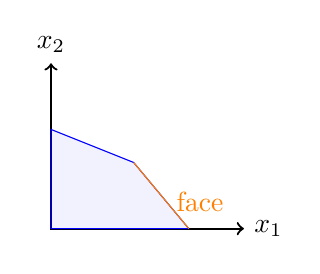
\begin{tikzpicture}[scale=0.7] % TODO: overlapping lines not pretty
        % axis
        \draw [<->, thick] (0,3) node (yaxis) [above] {$x_2$} |- (3.5,0) node (xaxis) [right] {$x_1$};
        % polygon
        \draw  [blue, fill=blue, fill opacity=0.05] (0.0, 1.8) -- (1.5, 1.2) -- (2.5, 0.0) -- (0,0) -- cycle;
        % face
        \draw [orange] (1.5, 1.2) -- node[pos=0.6, right] {face} (2.5, 0.0);

    \end{tikzpicture}
\end{frame}

% face is maximum
\begin{frame}{Characterisation of Faces}
    \begin{cor}
        For a polyhedron $P\coloneqq \{x\st Ax\leq b\}$ and a LP $\max\{c\cdot x\st x\in P\}$,
        the set of points attaining the maximum, are a face of $P$.
        \\
    \end{cor}
    TODO: tikz picture showing vertex and face as maxima.
\end{frame}


\section{Duality}
% duality
\begin{frame}{Duality Intuition}
    TODO: nice picture with inside/ outside distinction of LP and duality
\end{frame}

\begin{frame}{Duality Definition}
    \begin{defn}
        Given a LP $\max\{c\cdot x\st Ax\leq b\}$ (called the \textbf{primal LP}),
        the \textbf{dual LP} is the linear program $\min\{y\cdot b\st y^\top A =c, y\geq 0\}$.
    \end{defn}

\end{frame}

% duality prop & theorem
\begin{frame}{Duality}
    \begin{prop}
        The dual of the dual of an LP is (equivalent to) the primal LP.
    \end{prop}
    \pause
    \begin{theorem}[Duality Theorem]
        If the primal and it's dual LP are feasible, their solutions are the same. \\
        Formally: If $P\coloneqq\{x\st Ax\leq b\}$ and $D\coloneqq\{y\st y^\top A=c, y\geq 0\}$ are non empty,
        then \[\max\{c\cdot x\st x\in P\}=\min\{y\cdot b\st y\in D\}.\]
    \end{theorem}
\end{frame}

\begin{frame}{Duality}
    \begin{prop}[Weak Duality]
        Let $x$ and $y$ be feasible solutions of the LP's $\max\{c\cdot x \st Ax \leq b\}$
        and $\min\{y\cdot b\st y^\top A = c, y\geq 0\}$. % TODO: y * b => b * y
        Then $c\cdot x \leq y \cdot b$.
    \end{prop}
\end{frame}


\section[Simplex]{The Simplex Algorithm}

% simplex intuition
%\begin{frame}{Simplex Algorithm Intuition}
%    For $c=\begin{pmatrix*}0,0,1\end{pmatrix*}^\top$, and $P=\{x\st Ax\leq b\}$ a dodecahedron, the Simplex Algorithm does as follows:
%
%    TODO: picture of dodecaedron, walking optimal path from bottom vertex, to top.\\
%\end{frame}

\begin{frame}{Simplex Algorithm}
    Input: a linear program and a vertex of the polyhedron. \\
    Notation: $a_i \coloneqq A_{\{i\}}$ (the $i$'th row of $A$) \\
    Algorithm:
    \begin{enumerate}
        \item \label{step:1}Choose a set of n row indices $J$ such that $A_J$ is invertible and $A_{J}x = b_J$.
        \pause
        \item \label{step:2} Compute $c^\top (A_J)^{-1}$ and add zeros to obtain a vector $y$ with $c^\top = y^\top A$,
              such that all entries of $y$ outside $J$ are zero. \\
              \textbf{If} $y\geq 0$ \textbf{then stop. Return} $x$ and $y$.
        \pause
        \item  \label{step:3}Choose the minimum index $i$ with $y_i < 0$. \\
              Let $w$ be the column of $-(A_J)^{-1}$ with index $i$, so $A_{J\setminus\{i\}}w=0$
              and $a_i \cdot w = -1$.
        \pause
        \item \label{step:4}Let $\lambda \coloneqq \min  \set{\frac{b_j - a_j\cdot x}{a_j\cdot w} \st j\in\set{1,\dots, m}, a_j\cdot w > 0}$,
              and let $j$ be the smallest row index attaining this minimum.
        \pause
        \item \label{step:5} Set $J\coloneqq (J\setminus\set{i})\cup \set{j}$ and $x\coloneqq x + \lambda w$. \\
              \textbf{Go to}~\ref{step:2}.
    \end{enumerate}
\end{frame}

\begin{frame}{Simplex Algorithm Proof}
    \begin{proof}
        To follow closely, please refer to the algorithm on p. 57 of Combinatorial Optimization by Korte and Vygen. \\ %TODO: correct citation, make grey and italic?
        Invariants:
        \renewcommand{\theenumi}{(\alph{enumi})}
        \begin{multicols}{3}
        \begin{enumerate}  % TODO: labels
            \item $x \in P$
            \item $A_J x = b_J$
            \item $A_J$ invertible
            \item $c\cdot w > 0$
            \item $\lambda \geq 0$
        \end{enumerate}
        \end{multicols}

        % TODO: better enumeration of parts (out of order)
        (d): By step~\ref{step:2} $c^\top=y^\top A$
        $\Ra c\cdot w = c^\top w = (y^\top A)w = y^\top (Aw)$
        and by step~\ref{step:3} $A w = \colvec{0,\dots,-1,0,\dots,0}^\top$ \pause
        $\Ra y^\top (Aw) = -y_i > 0$ \pause  \\
        (e): By step~\ref{step:4} $a_j\cdot w > 0$ and if $x\in P$ then $b_i \geq a_i\cdot x$ \pause
        $\Ra \lambda = \frac{b_j-a_j\cdot x}{a_j\cdot w} \geq 0$ for chosen $j$. \\
    \end{proof}  % TODO: beamer proof no qed symbol (custom proof env without?)
\end{frame}

\begin{frame}{Simplex Algorithm Proof}
    \begin{proof}
    (c): $A_J$ invertible, is $A_{(J\setminus\set{i})\cup\set{j}}$? \\
         By step~\ref{step:3} $A_{J\setminus\set{i}} w = 0$ and $a_i w = -1$ for $w$ as $i$'th column of $-(A_J)^{-1}$.
         Iterate over $i$, get $-I_n$ (identity matrix). \pause \\
         After step~\ref{step:4} and~\ref{step:5} $i \leadsto j$ and $a_j w > 0$ $\Ra A_J$ invertible. \pause \\
    (b): show $x \in P \Ra x + \lambda w \in P$. Let $k$ be a row index.\\
         Two cases: % TODO: proper cases
         $a_k\cdot w \leq 0$\\
         $\Ra a_k\cdot (x+\lambda w) = a_k\cdot x + a_k\cdot w \leq a_k\cdot x \leq b_k$ \\
         $a_k \cdot w \geq 0$ \\
         Since $\lambda \coloneqq \min  \set{\frac{b_i - a_j\cdot x}{a_j\cdot w} \st j\in\set{1,\dots, m}, a_j\cdot w > 0}$ \\
         then $k$ in considered indices $\Ra \lambda \leq \frac{b_k - a_k\cdot x}{a_k\cdot w} $
         $\Ra a_k\cdot (x + \lambda w) \leq a_k\cdot x + \frac{b_k-a_k\cdot x}{a_k\cdot w} a_k\cdot w  = b_k$. \\
         Therefore in both cases $\Ra x+\lambda w \in P$.


    \end{proof}
\end{frame}

\begin{frame}{Simplex Algorithm Proof}
    \begin{proof}
        (a): After step~\ref{step:4} it holds that $A_{J\setminus\set{i}}w=0$ and $\lambda = \frac{b_j-a_j\cdot x}{a_j\cdot w}$
        $\Ra A_{J\setminus\set{i}}(x+\lambda w) = A_{J\setminus\set{i}}x + 0 = b_{J\setminus\set{i}}$
        and $\Ra a_j\cdot (x+\lambda w) = a_j \cdot w + \frac{b_j - a_j\cdot x}{a_j\cdot w} a_j\cdot w = b_j$. \\
        Thus $A_{(J\setminus\set{i})\cup\set{j}}(x+\lambda w) = b_{(J\setminus\set{i})\cup\set{j}}$.
    \end{proof}
\end{frame}


\end{document}
